\chapter{Triángulos y área hiperbólica}
\label{cap:triangulos-hiperbolicos}

La curvatura negativa se manifiesta de forma sencilla en los triángulos: la suma de sus ángulos interiores es menor que \(\pi\). La diferencia respecto al valor euclidiano determina el área del triángulo cuando la curvatura es \(-1\) \cite{anderson2005,greenberg2008}.

\section{Fórmula de área}

\begin{theorem}[Defecto angular]
Si un triángulo hiperbólico tiene ángulos interiores \(\alpha\), \(\beta\) y \(\gamma\), entonces
\begin{equation}
  \operatorname{Area}(T)=\pi-(\alpha+\beta+\gamma).
  \label{eq:area-triangulo}
\end{equation}
En particular, \(\alpha+\beta+\gamma<\pi\).
\end{theorem}

\begin{proof}
La fórmula es el caso triangular del teorema de Gauss--Bonnet para una superficie de curvatura constante \(-1\). El área coincide con el defecto angular, es decir, con la diferencia entre \(\pi\) y la suma de los ángulos interiores.
\end{proof}

\section{Triángulos ideales}

Un triángulo ideal tiene sus tres vértices en la frontera ideal. Sus vértices no son puntos del plano, pero los lados son geodésicas completas y el área es finita. Como los tres ángulos ideales son cero, su área es \(\pi\), de acuerdo con \cref{eq:area-triangulo}.

\begin{figure}[htbp]
  \centering
  % Triángulo ideal: vértices en la frontera y lados geodésicos ortogonales a ella.
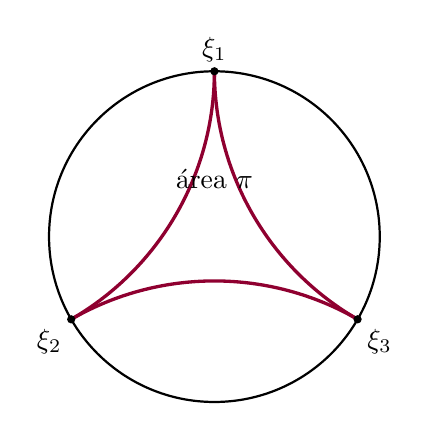
\begin{tikzpicture}[scale=2.1,line cap=round]
  \draw[thick] (0,0) circle (1cm);
  \draw[purple!75!black,very thick]
    (0,1) arc[start angle=0,end angle=-60,radius=1.7320508cm];
  \draw[purple!75!black,very thick]
    (0,1) arc[start angle=180,end angle=240,radius=1.7320508cm];
  \draw[purple!75!black,very thick]
    (-0.8660254,-0.5) arc[start angle=120,end angle=60,radius=1.7320508cm];
  \fill (0,1) circle (0.025) node[above] {$\xi_1$};
  \fill (-0.8660254,-0.5) circle (0.025) node[below left] {$\xi_2$};
  \fill (0.8660254,-0.5) circle (0.025) node[below right] {$\xi_3$};
  \node at (0,0.35) {área $\pi$};
\end{tikzpicture}

  \caption{Triángulo ideal en el disco de Poincaré. Los vértices están en la frontera ideal.}
  \label{fig:triangulo-ideal}
\end{figure}

\section{Ejercicios}

\begin{exercise}
Usa \cref{eq:area-triangulo} para calcular el área de un triángulo con ángulos \(\pi/2\), \(\pi/4\) y \(\pi/8\).
\end{exercise}

\begin{exercise}
Explica por qué la frontera circular dibujada en \cref{fig:triangulo-ideal} no representa una curva a distancia finita del interior.
\end{exercise}

\begin{remark}
La fórmula de área también funciona para polígonos geodésicos. Para un polígono de \(n\) lados, el área es \((n-2)\pi\) menos la suma de sus ángulos interiores.
\end{remark}
